% Options for packages loaded elsewhere
\PassOptionsToPackage{unicode}{hyperref}
\PassOptionsToPackage{hyphens}{url}
\PassOptionsToPackage{dvipsnames,svgnames*,x11names*}{xcolor}
%
\documentclass[
  ignorenonframetext,
]{beamer}
\usepackage{pgfpages}
\setbeamertemplate{caption}[numbered]
\setbeamertemplate{caption label separator}{: }
\setbeamercolor{caption name}{fg=normal text.fg}
\beamertemplatenavigationsymbolsempty
% Prevent slide breaks in the middle of a paragraph
\widowpenalties 1 10000
\raggedbottom
\setbeamertemplate{part page}{
  \centering
  \begin{beamercolorbox}[sep=16pt,center]{part title}
    \usebeamerfont{part title}\insertpart\par
  \end{beamercolorbox}
}
\setbeamertemplate{section page}{
  \centering
  \begin{beamercolorbox}[sep=12pt,center]{part title}
    \usebeamerfont{section title}\insertsection\par
  \end{beamercolorbox}
}
\setbeamertemplate{subsection page}{
  \centering
  \begin{beamercolorbox}[sep=8pt,center]{part title}
    \usebeamerfont{subsection title}\insertsubsection\par
  \end{beamercolorbox}
}
\AtBeginPart{
  \frame{\partpage}
}
\AtBeginSection{
  \ifbibliography
  \else
    \frame{\sectionpage}
  \fi
}
\AtBeginSubsection{
  \frame{\subsectionpage}
}
\usepackage{lmodern}
\usepackage{amssymb,amsmath}
\usepackage{ifxetex,ifluatex}
\ifnum 0\ifxetex 1\fi\ifluatex 1\fi=0 % if pdftex
  \usepackage[T1]{fontenc}
  \usepackage[utf8]{inputenc}
  \usepackage{textcomp} % provide euro and other symbols
\else % if luatex or xetex
  \usepackage{unicode-math}
  \defaultfontfeatures{Scale=MatchLowercase}
  \defaultfontfeatures[\rmfamily]{Ligatures=TeX,Scale=1}
\fi
% Use upquote if available, for straight quotes in verbatim environments
\IfFileExists{upquote.sty}{\usepackage{upquote}}{}
\IfFileExists{microtype.sty}{% use microtype if available
  \usepackage[]{microtype}
  \UseMicrotypeSet[protrusion]{basicmath} % disable protrusion for tt fonts
}{}
\makeatletter
\@ifundefined{KOMAClassName}{% if non-KOMA class
  \IfFileExists{parskip.sty}{%
    \usepackage{parskip}
  }{% else
    \setlength{\parindent}{0pt}
    \setlength{\parskip}{6pt plus 2pt minus 1pt}}
}{% if KOMA class
  \KOMAoptions{parskip=half}}
\makeatother
\usepackage{xcolor}
\IfFileExists{xurl.sty}{\usepackage{xurl}}{} % add URL line breaks if available
\IfFileExists{bookmark.sty}{\usepackage{bookmark}}{\usepackage{hyperref}}
\hypersetup{
  pdftitle={Modeling with Probability Distributions - Capturing Noise},
  pdfauthor={Zack Treisman},
  colorlinks=true,
  linkcolor=Maroon,
  filecolor=Maroon,
  citecolor=blue,
  urlcolor=Blue,
  pdfcreator={LaTeX via pandoc}}
\urlstyle{same} % disable monospaced font for URLs
\newif\ifbibliography
\usepackage{color}
\usepackage{fancyvrb}
\newcommand{\VerbBar}{|}
\newcommand{\VERB}{\Verb[commandchars=\\\{\}]}
\DefineVerbatimEnvironment{Highlighting}{Verbatim}{commandchars=\\\{\}}
% Add ',fontsize=\small' for more characters per line
\usepackage{framed}
\definecolor{shadecolor}{RGB}{248,248,248}
\newenvironment{Shaded}{\begin{snugshade}}{\end{snugshade}}
\newcommand{\AlertTok}[1]{\textcolor[rgb]{0.94,0.16,0.16}{#1}}
\newcommand{\AnnotationTok}[1]{\textcolor[rgb]{0.56,0.35,0.01}{\textbf{\textit{#1}}}}
\newcommand{\AttributeTok}[1]{\textcolor[rgb]{0.77,0.63,0.00}{#1}}
\newcommand{\BaseNTok}[1]{\textcolor[rgb]{0.00,0.00,0.81}{#1}}
\newcommand{\BuiltInTok}[1]{#1}
\newcommand{\CharTok}[1]{\textcolor[rgb]{0.31,0.60,0.02}{#1}}
\newcommand{\CommentTok}[1]{\textcolor[rgb]{0.56,0.35,0.01}{\textit{#1}}}
\newcommand{\CommentVarTok}[1]{\textcolor[rgb]{0.56,0.35,0.01}{\textbf{\textit{#1}}}}
\newcommand{\ConstantTok}[1]{\textcolor[rgb]{0.00,0.00,0.00}{#1}}
\newcommand{\ControlFlowTok}[1]{\textcolor[rgb]{0.13,0.29,0.53}{\textbf{#1}}}
\newcommand{\DataTypeTok}[1]{\textcolor[rgb]{0.13,0.29,0.53}{#1}}
\newcommand{\DecValTok}[1]{\textcolor[rgb]{0.00,0.00,0.81}{#1}}
\newcommand{\DocumentationTok}[1]{\textcolor[rgb]{0.56,0.35,0.01}{\textbf{\textit{#1}}}}
\newcommand{\ErrorTok}[1]{\textcolor[rgb]{0.64,0.00,0.00}{\textbf{#1}}}
\newcommand{\ExtensionTok}[1]{#1}
\newcommand{\FloatTok}[1]{\textcolor[rgb]{0.00,0.00,0.81}{#1}}
\newcommand{\FunctionTok}[1]{\textcolor[rgb]{0.00,0.00,0.00}{#1}}
\newcommand{\ImportTok}[1]{#1}
\newcommand{\InformationTok}[1]{\textcolor[rgb]{0.56,0.35,0.01}{\textbf{\textit{#1}}}}
\newcommand{\KeywordTok}[1]{\textcolor[rgb]{0.13,0.29,0.53}{\textbf{#1}}}
\newcommand{\NormalTok}[1]{#1}
\newcommand{\OperatorTok}[1]{\textcolor[rgb]{0.81,0.36,0.00}{\textbf{#1}}}
\newcommand{\OtherTok}[1]{\textcolor[rgb]{0.56,0.35,0.01}{#1}}
\newcommand{\PreprocessorTok}[1]{\textcolor[rgb]{0.56,0.35,0.01}{\textit{#1}}}
\newcommand{\RegionMarkerTok}[1]{#1}
\newcommand{\SpecialCharTok}[1]{\textcolor[rgb]{0.00,0.00,0.00}{#1}}
\newcommand{\SpecialStringTok}[1]{\textcolor[rgb]{0.31,0.60,0.02}{#1}}
\newcommand{\StringTok}[1]{\textcolor[rgb]{0.31,0.60,0.02}{#1}}
\newcommand{\VariableTok}[1]{\textcolor[rgb]{0.00,0.00,0.00}{#1}}
\newcommand{\VerbatimStringTok}[1]{\textcolor[rgb]{0.31,0.60,0.02}{#1}}
\newcommand{\WarningTok}[1]{\textcolor[rgb]{0.56,0.35,0.01}{\textbf{\textit{#1}}}}
\usepackage{graphicx,grffile}
\makeatletter
\def\maxwidth{\ifdim\Gin@nat@width>\linewidth\linewidth\else\Gin@nat@width\fi}
\def\maxheight{\ifdim\Gin@nat@height>\textheight\textheight\else\Gin@nat@height\fi}
\makeatother
% Scale images if necessary, so that they will not overflow the page
% margins by default, and it is still possible to overwrite the defaults
% using explicit options in \includegraphics[width, height, ...]{}
\setkeys{Gin}{width=\maxwidth,height=\maxheight,keepaspectratio}
% Set default figure placement to htbp
\makeatletter
\def\fps@figure{htbp}
\makeatother
\setlength{\emergencystretch}{3em} % prevent overfull lines
\providecommand{\tightlist}{%
  \setlength{\itemsep}{0pt}\setlength{\parskip}{0pt}}
\setcounter{secnumdepth}{-\maxdimen} % remove section numbering

\pgfdeclareimage[width=3.5cm]{mcslogo}{../western_logo_hor_MCS_3C_pos.pdf}
\pgfdeclareimage[width=1cm]{ccbysa}{../ccbysa88x31.png}
\titlegraphic{\href{http://creativecommons.org/licenses/by-sa/4.0/}{\pgfuseimage{ccbysa}}
\hfill
\href{https://western.edu/program/mathematics/}{\pgfuseimage{mcslogo}}}
%\usecolortheme{wcu}
%\institute{Western Colorado University}
%\setbeamertemplate{navigation symbols}{}

\title{Modeling with Probability Distributions - Capturing Noise}
\author{Zack Treisman}
\date{Spring 2021}

\begin{document}
\frame{\titlepage}

\begin{frame}{Philosophy}
\protect\hypertarget{philosophy}{}

Recall that a model fundamentally looks like \[
y=f(x)+\epsilon
\] where \(f(x)\) is the \textbf{deterministic} part of the model (the
signal) and \(\epsilon\) is the \textbf{stochastic} part (the noise).

\begin{itemize}
\tightlist
\item
  This week we are looking at the \textbf{noise}.
\end{itemize}

We'll look at the how to model noise in the general context of studying
probability, and we'll lay some groundwork for some additional
applications of probability.

The noise is a probability distribution. So far, we have only considered
models where the noise follows a normal (Gaussian) distribution.
Choosing the best distribution is an important part of the modeling
process.

\end{frame}

\begin{frame}{Breaking up the noise}
\protect\hypertarget{breaking-up-the-noise}{}

We have already talked about how the noise can be broken into
irreducible and reducible error, and the reducible error can be split
into bias and variance. This decomposition is model based.

Another way that the noise can be decomposed is more observation based:

\begin{itemize}
\tightlist
\item
  Measurement error - Unavoidable, but hopefully minimal. If it has
  structure or pattern, this can cause difficulties, some of which can
  be overcome (eg. distance sampling).
\item
  Process noise - Natural demographic and environmental variability.
  Minimized with large samples and stable environments. The main input
  to the stochastic part of a model.
\end{itemize}

\end{frame}

\begin{frame}{Conditional distributions}
\protect\hypertarget{conditional-distributions}{}

A more computationally convenient phrasing and notation than
\(y=f(x)+\epsilon\) is to describe noise as a \textbf{conditional
distribution}.

\[
Y\sim \mathbb{P}(f(X))
\]

\begin{itemize}
\tightlist
\item
  \(f(X)\) represents the expected value of \(Y\) as a function of
  \(X\).
\item
  \(\mathbb{P}\) can be any distribution.
\end{itemize}

A model where applying a link function to \(f\) makes it linear in its
parameters is called a \textbf{generalized linear model} (GLM). Somewhat
more general \(f\) can be fit with a \textbf{generalized additive model}
(GAM).

\end{frame}

\begin{frame}[fragile]{The \texttt{glm} and related commands}
\protect\hypertarget{the-glm-and-related-commands}{}

Fitting generalized linear models in R is done using \texttt{glm},
generalized additive models with \texttt{gam}.

\begin{Shaded}
\begin{Highlighting}[]
\NormalTok{?glm}

\KeywordTok{glm}\NormalTok{(formula, }\DataTypeTok{family =}\NormalTok{ gaussian, data,}
\NormalTok{    na.action, }\DataTypeTok{start =} \OtherTok{NULL}\NormalTok{, ...)}

\NormalTok{?family}

\KeywordTok{binomial}\NormalTok{(}\DataTypeTok{link =} \StringTok{"logit"}\NormalTok{)}
\KeywordTok{gaussian}\NormalTok{(}\DataTypeTok{link =} \StringTok{"identity"}\NormalTok{)}
\KeywordTok{Gamma}\NormalTok{(}\DataTypeTok{link =} \StringTok{"inverse"}\NormalTok{)}
\KeywordTok{inverse.gaussian}\NormalTok{(}\DataTypeTok{link =} \StringTok{"1/mu^2"}\NormalTok{)}
\KeywordTok{poisson}\NormalTok{(}\DataTypeTok{link =} \StringTok{"log"}\NormalTok{)}
\NormalTok{...}
\end{Highlighting}
\end{Shaded}

\end{frame}

\hypertarget{probability}{%
\section{Probability}\label{probability}}

\begin{frame}{Definitions and notation}
\protect\hypertarget{definitions-and-notation}{}

The \textbf{sample space} is the set of all possible \textbf{outcomes}.
Each opportunity for an outcome to occur is a \textbf{trial}. Outcomes
are collected into \textbf{events}. To each event \(A\) we assign a
number \(P(A)\) between 0 and 1 called the \textbf{probability} of \(A\)
representing the frequency with which \(A\) occurs.

\footnotesize

Example: A feeder at my house is visited by various birds and mammals.
Each visit is a trial. The set of all critters that visit the feeder is
the sample space. A grey jay visiting is an event. By my estimation
\(P(\text{Grey Jay})=0.3\). One of the grey jays that visits I've named
June. June visiting the feeder is an outcome.

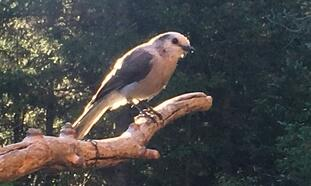
\includegraphics[width=\textwidth,height=0.4\textheight]{grey_jay.jpg}

\end{frame}

\begin{frame}{Notation}
\protect\hypertarget{notation}{}

Let \(A\) and \(B\) be events from a sample space \(S\).

\begin{itemize}
\tightlist
\item
  \(A\) \emph{or} \(B\) is written \(A\cup B\). (Inclusive or: \(A\) or
  \(B\) or both.)
\item
  \(A\) \emph{and} \(B\) is written \(A\cap B\).
\item
  The \textbf{conditional probability} of \(A\) given \(B\), written
  \(P(A|B)\), is the probability that \(A\) happens if \(B\) is known to
  happen.
\end{itemize}

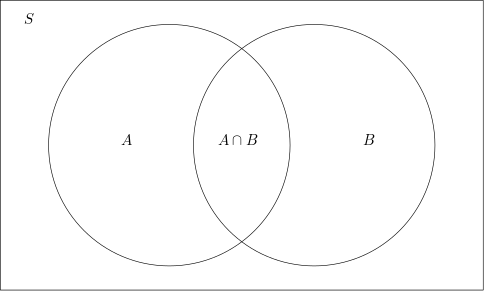
\includegraphics[width=\textwidth,height=0.5\textheight]{../images/AB.png}

\end{frame}

\begin{frame}{Axioms of probability}
\protect\hypertarget{axioms-of-probability}{}

The mathematics of probability can be derived from the following three
algebraic axioms.

\begin{enumerate}
\item
  \(P(S)=1\): Something has to happen.
\item
  \(P(A\cup B)=P(A)+P(B)-P(A\cap B)\): The probability of either or both
  of \(A\) or \(B\) happening is the sum of their individual
  probabilities, less the probability that both happen (which was
  counted twice in the sum).
\item
  \(\displaystyle P(A|B)=\frac{P(A\cap B)}{P(B)}\): The probability that
  \(A\) happens given that \(B\) has happened can be computed by
  rescaling the probability that both \(A\) and \(B\) happen by the
  probability of \(B\).
\end{enumerate}

\end{frame}

\begin{frame}{Algebra of probability}
\protect\hypertarget{algebra-of-probability}{}

Some immediate consequences of the axioms that are very useful are the
following.

\begin{itemize}
\tightlist
\item
  Since \(S=A\cup(\text{not }A)\), combining rules 1 and 2 gives that
  the probability that \(A\) doesn't happen is
  \(P(\text{not }A)=1-P(A)\).
\item
  More generally, if \(A\) and \(B\) are any mutually exclusive events,
  \(P(A\cup B)=P(A)+P(B)\).
\item
  The unconditional probability of an event can be computed by making
  use of known conditional probabilities:
  \(P(A)=P(A|B)P(B)+P(A|\text{not }B)P(\text{not }B)\)
\item
  If \(P(A)=P(A|B)\) we say that \(A\) and \(B\) are
  \textbf{independent}. In this situation, rule 3 implies that
  \(P(A\cap B)=P(A)P(B)\).
\end{itemize}

\end{frame}

\begin{frame}{Application: Zero-inflated distributions}
\protect\hypertarget{application-zero-inflated-distributions}{}

Consider the seed predation example from Bolker (2008):

A feeder has \(N\) seeds. The sample space is the number of seeds taken
between occasions when the feeder is checked, so the numbers between
\(0\) and \(N\).

On many occasions, no seeds are taken, in which case it is reasonable to
assume that the feeder may not have been visited.

\begin{itemize}
\tightlist
\item
  \(P(\text{feeder is visited})=\nu\).
\end{itemize}

Assume that a visitor to the feeder independently considers taking each
seed.

\begin{itemize}
\tightlist
\item
  \(P(\text{seed taken})=p\).
\end{itemize}

\end{frame}

\begin{frame}{Application: Zero-inflated distributions (cont.)}
\protect\hypertarget{application-zero-inflated-distributions-cont.}{}

If no seeds are taken that means that either nobody visited \[
P(\text{no visit})=1-\nu
\] or a visitor came \[
P(\text{visit})=\nu
\] and decided not to take each seed \begin{align*}
P(\text{not seed 1}\cap\cdots\cap\text{not seed }N) &= P(\text{not seed 1})\cdots P(\text{not seed }N)\\
&= (1-p)^N
\end{align*} Putting these together gives \[
P(\text{no seeds taken})=1-\nu+\nu(1-p)^N
\]

\end{frame}

\begin{frame}{Application: Zero-inflated distributions (cont. 2)}
\protect\hypertarget{application-zero-inflated-distributions-cont.-2}{}

On the other hand, the event that \(x\) seeds are taken consists of \[
{N\choose x}=\frac{N!}{x!(N-x)!}
\] different outcomes (one for each way to select \(x\) of \(N\) seeds)
each with probability \[
p^x(1-p)^{N-x}
\] So for \(x>0\), \[
P(x\text{ seeds taken})=\nu{N\choose x}p^x(1-p)^{N-x}
\] The distribution that we have just derived is called the
\textbf{zero-inflated binomial}. Other zero-inflated models are similar,
and can be very useful in ecological applications.

\end{frame}

\begin{frame}[fragile]{Zero-inflated binomial in R}
\protect\hypertarget{zero-inflated-binomial-in-r}{}

This code defines and plots a zero-inflated binomial model. See Figure
4.1 in Bolker. \scriptsize

\begin{Shaded}
\begin{Highlighting}[]
\NormalTok{N <-}\DecValTok{10} \CommentTok{# number of seeds per feeder}
\NormalTok{nu <-}\StringTok{ }\FloatTok{0.8} \CommentTok{# visit probability}
\NormalTok{p <-}\StringTok{ }\FloatTok{0.3} \CommentTok{# probability of taking each individual seed}
\NormalTok{dzibinom <-}\StringTok{ }\KeywordTok{numeric}\NormalTok{(N}\OperatorTok{+}\DecValTok{1}\NormalTok{) }\CommentTok{# Initialize an empty vector of length N+1}
\NormalTok{dzibinom[}\DecValTok{1}\NormalTok{] <-}\StringTok{ }\DecValTok{1}\OperatorTok{-}\NormalTok{nu}\OperatorTok{+}\NormalTok{nu}\OperatorTok{*}\NormalTok{(}\DecValTok{1}\OperatorTok{-}\NormalTok{p)}\OperatorTok{^}\NormalTok{N }\CommentTok{# Zero seeds taken}
\ControlFlowTok{for}\NormalTok{(x }\ControlFlowTok{in} \DecValTok{1}\OperatorTok{:}\NormalTok{N) \{ }\CommentTok{# x seeds taken}
\NormalTok{  dzibinom[x}\OperatorTok{+}\DecValTok{1}\NormalTok{] <-nu}\OperatorTok{*}\KeywordTok{choose}\NormalTok{(N,x)}\OperatorTok{*}\NormalTok{p}\OperatorTok{^}\NormalTok{x}\OperatorTok{*}\NormalTok{(}\DecValTok{1}\OperatorTok{-}\NormalTok{p)}\OperatorTok{^}\NormalTok{(N}\OperatorTok{-}\NormalTok{x)\}}
\KeywordTok{barplot}\NormalTok{(dzibinom, }\DataTypeTok{names.arg=}\DecValTok{0}\OperatorTok{:}\NormalTok{N, }\DataTypeTok{xlab=}\StringTok{"Taken"}\NormalTok{, }\DataTypeTok{ylab=}\StringTok{"Probability"}\NormalTok{)}
\end{Highlighting}
\end{Shaded}

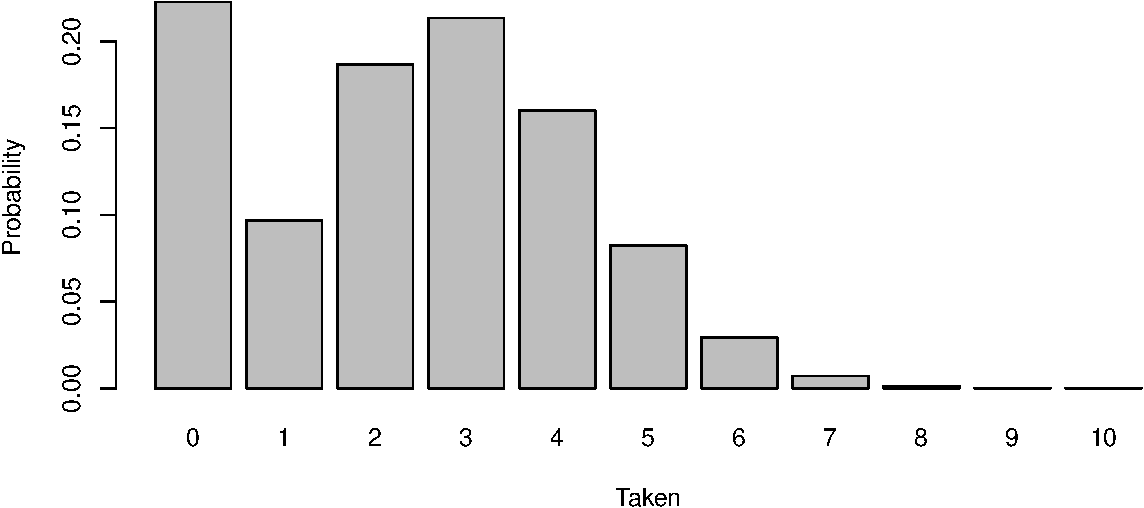
\includegraphics{noise_files/figure-beamer/unnamed-chunk-3-1.pdf}

\end{frame}

\hypertarget{bayes-rule-and-bayesian-statistics}{%
\section{Bayes' Rule and Bayesian
Statistics}\label{bayes-rule-and-bayesian-statistics}}

\begin{frame}{Bayes Rule}
\protect\hypertarget{bayes-rule}{}

Bayes' Rule allows us to reverse the conditionality in probability
calculations. For any events \(A\) and \(B\): \[
P(A|B)=\frac{P(B|A)P(A)}{P(B)}
\] Turning the conditionality around is useful for hypothesis testing.

\begin{itemize}
\tightlist
\item
  Hypothesis: \(A\); Observed Data: \(B\)
\item
  \(P(A|B)\) is the probability that the hypothesis is true given the
  observed data. (What we want to know.)
\item
  Everything on the right side we can calculate from assumptions in the
  hypothesis and observations of the data.
\end{itemize}

\end{frame}

\begin{frame}{Derivation of Bayes' Rule}
\protect\hypertarget{derivation-of-bayes-rule}{}

Before we talk about how to use it, let's take a second to algebraically
justify the rule. Going from the axioms of probability to Bayes' Rule is
satisfyingly easy:

First, \(A\cap B = B\cap A\) are just two ways of writing the same event
``\(A\) and \(B\)''. Second, rephrasing axiom 3 above gives \[
P(A\cap B) = P(A|B)P(B)
\] and \[
P(B\cap A)=P(B|A)P(A).
\] Thus \[
P(A|B)P(B)=P(B|A)P(A)
\] and dividing both sides by \(P(B)\) gives Bayes' Rule.

\end{frame}

\begin{frame}{From Bayes' Rule to Bayesian statistics}
\protect\hypertarget{from-bayes-rule-to-bayesian-statistics}{}

\footnotesize

Bayes' Rule applied to observed data \(D\) and hypothesis \(H\): \[
P(H|D)=\frac{P(D|H)P(H)}{P(D)}
\] We want the left hand side. What can we do with the three terms on
the right?

\begin{itemize}
\tightlist
\item
  \(P(D|H)\): Called the \textbf{likelihood} of the data.

  \begin{itemize}
  \tightlist
  \item
    \(H\) gives a distribution for calculating \(P(\text{datum}|H)\).
  \item
    Independent data means
    \(P(D|H)=\prod_{\text{datum}\in D} P(\text{datum}|H)\).
  \item
    Often calculate \emph{log likelihoods} in practice.
  \end{itemize}
\item
  \(P(H)\): This is called the \textbf{prior}.

  \begin{itemize}
  \tightlist
  \item
    Assumed before looking at the data.
  \item
    Choosing appropriate priors can be difficult and controversial.
  \item
    Default to \emph{uninformative} or \emph{uniform} priors.
  \end{itemize}
\item
  \(P(D)\): Using a set \(H_1\) to \(H_N\) of \emph{exhaustive, mutually
  exclusive} hypotheses: \begin{align*}
  P(D) & = \sum_{j=1}^N P(D\cap H_j)\\
  & =  \sum_{j=1}^N P(D|H_j)P(H_j)
  \end{align*}
\end{itemize}

\end{frame}

\begin{frame}{Bayes' Rule: Example}
\protect\hypertarget{bayes-rule-example}{}

\begin{itemize}
\tightlist
\item
  Disease with prevalence of 10 per 100,000.
\item
  Test that is 99\% accurate. (For both positive and negative results;
  these could also be different.)
\end{itemize}

Two questions: Given a positive test result how likely is it that the
subject is sick (sensitivity), and given a negative result, how likely
is it that the subject is healthy (specificity)?

\begin{itemize}
\tightlist
\item
  We'll calculate the sensitivity:
\end{itemize}

\scriptsize

\begin{align*}
P(\text{sick}|\text{test}+) & = \frac{P(\text{test}+|\text{sick})P(\text{sick})}{P(\text{test}+)} \\
      & = \frac{P(\text{test}+|\text{sick})P(\text{sick})}
      {P(\text{test}+|\text{sick})P(\text{sick})+P(\text{test}+|\text{not sick})P(\text{not sick})} \\
      & = \frac{0.99 \times 0.00001}{0.99 \times 0.00001 + 0.01 \times 0.99999}\\
      & \approx 0.001
\end{align*}

\normalsize

So this 99\% accurate test is not \emph{nearly} sensitive enough for
reliably detecting cases of this disease.

\end{frame}

\hypertarget{distributions}{%
\section{Distributions}\label{distributions}}

\begin{frame}[fragile]{Definitions and notation}
\protect\hypertarget{definitions-and-notation-1}{}

Let \(X\) be a random variable. Traditional notation uses \(X\) for the
variable and \(x\) for particular values.

``I worried for a long time about what the term `random variable' means.
In the end I concluded it means: `variable'.'' -J.H.Conway

\begin{itemize}
\tightlist
\item
  The \textbf{probability distribution function} of \(X\) tells us the
  probability that \(X\) takes a particular value.

  \begin{itemize}
  \tightlist
  \item
    \(X\) discrete: \(f(x)=P(X=x)\)
  \item
    \(X\) continuous: \(\int_a^b f(x) dx = P(a\leq X\leq b)\)
  \end{itemize}
\item
  The \textbf{cumulative distribution function} of \(X\) is
  \(F(x)=P(X\leq x)\).
\end{itemize}

R has many distributions built in. See \texttt{?Distributions}.

\end{frame}

\begin{frame}{Moments}
\protect\hypertarget{moments}{}

A probability distribution defines an \textbf{expectation} operation. \[
E[z]=\sum_x z f(x) \text{ or } E[z]=\int z f(x) dx.
\]

\begin{itemize}
\tightlist
\item
  \(E[x]=\mu=\bar x\) is the \textbf{mean}.
\item
  \(E[(x-\bar x)^2]=\sigma^2\) is the \textbf{variance}.
\end{itemize}

Continuing in a similar way defines the \textbf{skewness} and
\textbf{kurtosis} (heavy-tailedness). If you need to numerically measure
these things you are probably doing something fancy and mathematically
impressive.

\textbf{Method of moments}: To choose a particular distribution from an
assumed family, calculate moments for data and use these to compute
appropriate parameters.

\end{frame}

\begin{frame}{Binomial}
\protect\hypertarget{binomial}{}

\(X\): The number of successes after repeated independent and identical
trials.

Parameters are \(N\), the number of trials, and \(p\), the probability
of success on each trial.

\begin{itemize}
\tightlist
\item
  Discrete, defined for \(0\leq x \leq N\)
\item
  \(f(x)={N\choose x}p^x(1-p)^{N-x}\)
\item
  \(\mu=Np\), \(\sigma^2=Np(1-p)\)
\end{itemize}

Approximately normal for large \(N\), intermediate \(p\). Approximately
Poisson for large \(N\), small \(p\).

\end{frame}

\begin{frame}[fragile]{Binomial example}
\protect\hypertarget{binomial-example}{}

Suppose 10\% of red foxes have the cross fox color variation. How many
cross foxes would we expect in a sample of size \(N\)?

\scriptsize

\begin{Shaded}
\begin{Highlighting}[]
\NormalTok{N <-}\StringTok{ }\DecValTok{25}
\NormalTok{p <-}\StringTok{ }\FloatTok{0.1}
\KeywordTok{barplot}\NormalTok{(}\KeywordTok{dbinom}\NormalTok{(}\DecValTok{0}\OperatorTok{:}\NormalTok{N, N, p), }
        \DataTypeTok{names.arg=}\DecValTok{0}\OperatorTok{:}\NormalTok{N, }\DataTypeTok{xlab=}\StringTok{"cross foxes"}\NormalTok{, }\DataTypeTok{ylab=}\StringTok{"Probability"}\NormalTok{)}
\KeywordTok{lines}\NormalTok{(}\KeywordTok{dpois}\NormalTok{(}\DecValTok{0}\OperatorTok{:}\NormalTok{N, N}\OperatorTok{*}\NormalTok{p), }\DataTypeTok{col=}\StringTok{"red"}\NormalTok{) }\CommentTok{# Poisson approximation}
\end{Highlighting}
\end{Shaded}

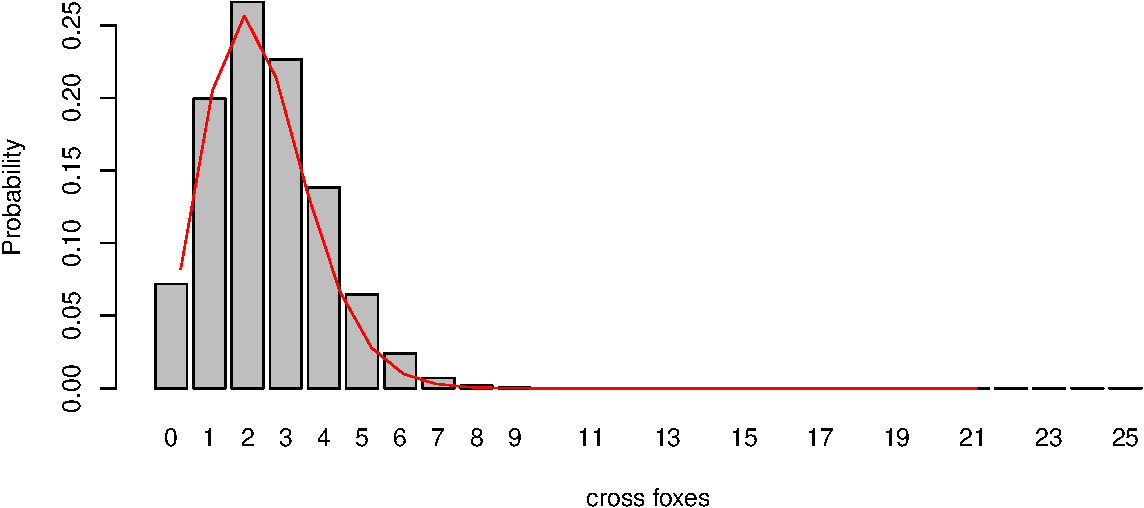
\includegraphics{noise_files/figure-beamer/unnamed-chunk-4-1.pdf}

\end{frame}

\begin{frame}{Poisson}
\protect\hypertarget{poisson}{}

\(X\): The count of observations of an evenly distributed event in a
given time/space/unit of counting effort.

Parameter is \(\lambda\), the expected count.

\begin{itemize}
\tightlist
\item
  Discrete, defined for \(0\leq x\)
\item
  \(\displaystyle f(x)=\frac{e^{-\lambda}\lambda^x}{x!}\)
\item
  \(\mu=\lambda\), \(\sigma^2=\lambda\)
\end{itemize}

Right skewed. Approximately normal for large \(\lambda\).

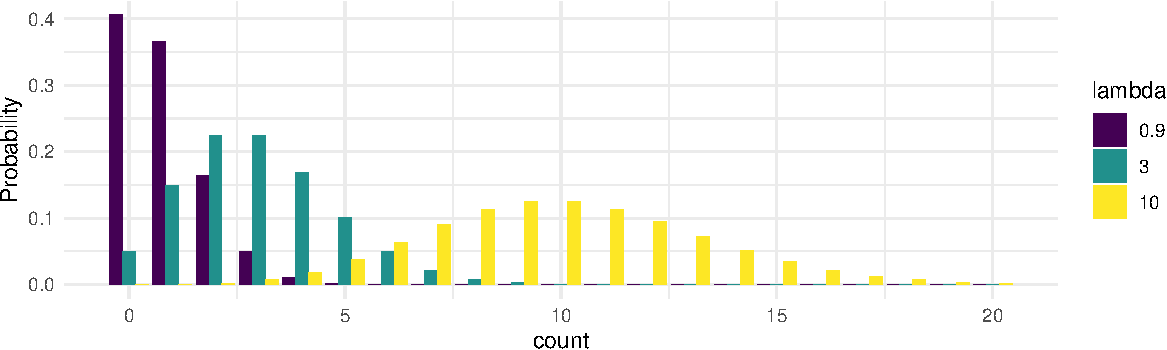
\includegraphics{noise_files/figure-beamer/unnamed-chunk-5-1.pdf}

\end{frame}

\begin{frame}{Negative Binomial}
\protect\hypertarget{negative-binomial}{}

\(X\): Similar to Poisson, but the events can be clustered.

Parameters are \(\mu\), the expected count, and \(k\), the
overdispersion parameter. Smaller \(k\) means more clustering.

\begin{itemize}
\tightlist
\item
  Discrete, defined for \(0\leq x\)
\item
  \(\displaystyle f(x)=\frac{\Gamma(k+x)}{\Gamma(k)x!}\left(\frac{k}{k+\mu}\right)^k\left(\frac{\mu}{k+\mu}\right)^x\)
\item
  \(\mu=\mu\), \(\sigma^2=\mu+\mu^2/k\)
\end{itemize}

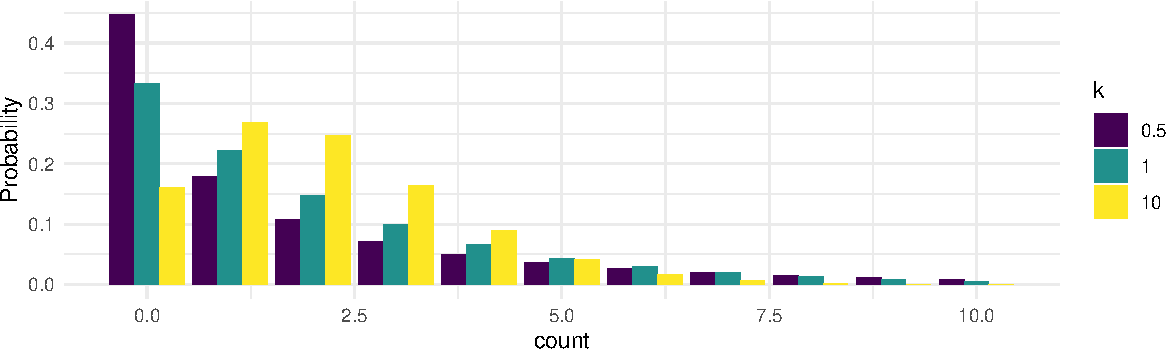
\includegraphics{noise_files/figure-beamer/unnamed-chunk-6-1.pdf}

Alternatively \(X\): count of failures before a fixed number of
successes.

\end{frame}

\begin{frame}{Uniform}
\protect\hypertarget{uniform}{}

The most boring distribution. \(X\) from \(U(a,b)\) means all values
between the lower limit \(a\) and upper limit \(b\) are equally likely.

\begin{itemize}
\tightlist
\item
  Generally continuous. Could be discrete depending on context.
\end{itemize}

\end{frame}

\begin{frame}{Normal}
\protect\hypertarget{normal}{}

\(X\): The sum of many independent samples.

Parameters mean \(\mu\) and variance \(\sigma^2\) (or standard deviation
\(\sigma\)). Write \(N(\mu, \sigma^2)\).

\begin{itemize}
\tightlist
\item
  Continuous, defined for all real numbers \(x\)
\item
  \(f(x)=\displaystyle \frac{1}{\sigma\sqrt{2\pi}}\exp\left(-\frac{1}{2}\left(\frac{x-\mu}{\sigma}\right)^2\right)\)
\end{itemize}

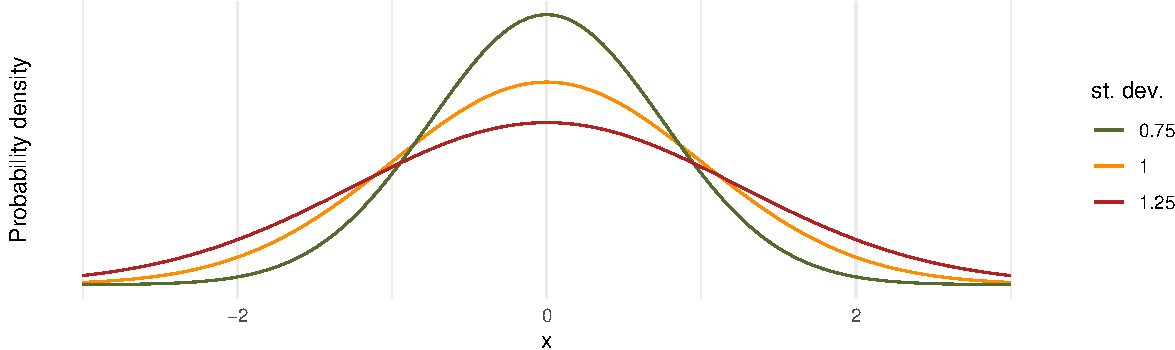
\includegraphics{noise_files/figure-beamer/unnamed-chunk-7-1.pdf}

The gold standard for noise. Most classical statistical techniques rely
on assuming that the noise is normal.

\end{frame}

\begin{frame}{Gamma}
\protect\hypertarget{gamma}{}

\(X\): The waiting time until a set number of events take place.

Parameters scale \(s\), the length per event, or rate \(r=1/s\), the
rate at which events occur, and shape \(a\), the number of events.

\begin{itemize}
\tightlist
\item
  Continuous, \(x\geq 0\)
\item
  \(f(x)=\frac{1}{s^a\Gamma(a)}x^{a-1}e^{-x/s}\)
\item
  \(\mu=as\), \(\sigma^2=as^2\)
\end{itemize}

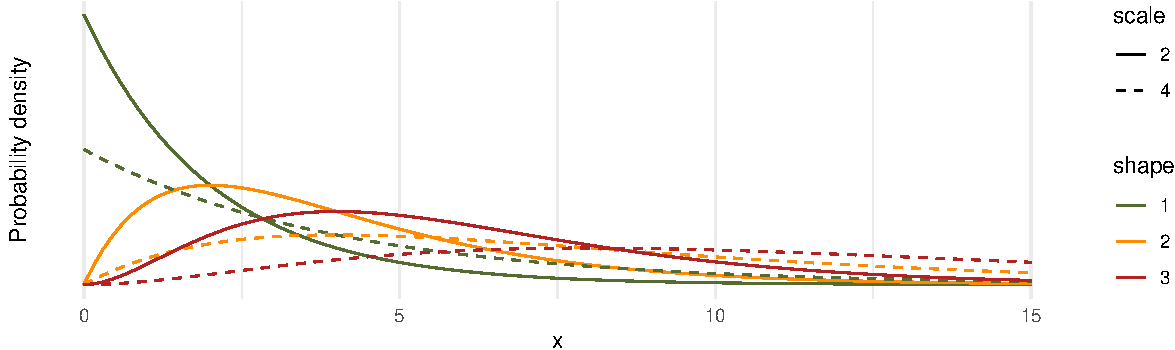
\includegraphics{noise_files/figure-beamer/unnamed-chunk-8-1.pdf}

Along with the log-normal, also used for models needing a continuous,
right skewed, non-negative distribution without necessarily having a
mechanistic reason.

\end{frame}

\begin{frame}{Log-normal}
\protect\hypertarget{log-normal}{}

\(X\): The product of many independent samples.

Parameters mean of the log \(\mu\) and standard deviation of the log
\(\sigma\).

\begin{itemize}
\tightlist
\item
  Continuous, \(x>0\)
\item
  \(X\sim \exp(\mu+\sigma Z)\) for \(Z\sim N(0,1)\).
\end{itemize}

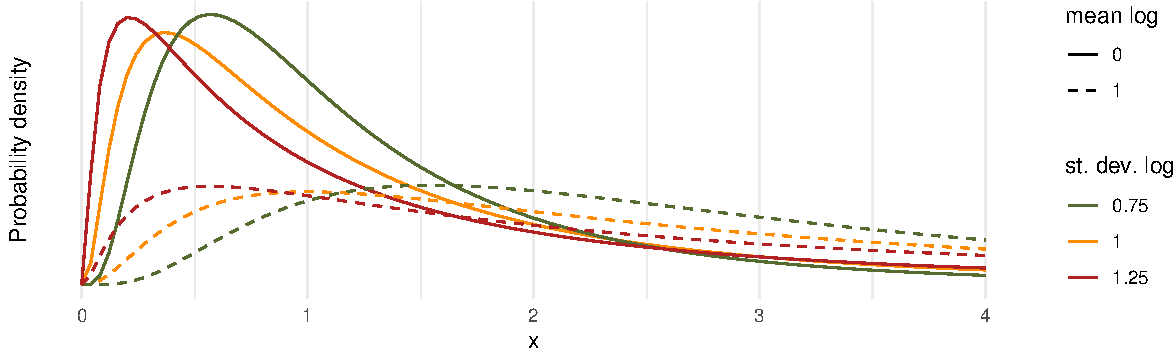
\includegraphics{noise_files/figure-beamer/unnamed-chunk-9-1.pdf}

Recall that the mean is \(\exp(\mu+\sigma^2/2)\).

\end{frame}

\begin{frame}{Mixtures and compounded distributions}
\protect\hypertarget{mixtures-and-compounded-distributions}{}

Sometimes it is useful to combine distributions or allow the parameters
of a distribution be drawn from another distribution. For example, the
effects of unknown or unmeasured variables, can potentially be captured
by such a varying parameter.

Combining a finite number of distributions into a single distribution is
called a \textbf{mixture distribution}. The zero-inflated binomial that
we created earlier is an example.

Drawing a parameter of one distribution from a second is called a
\textbf{compound distribution}. Drawing the rate parameter \(\lambda\)
for a Poisson distribution from a Gamma distribution gives a negative
binomial distribution.

\end{frame}

\begin{frame}{References}
\protect\hypertarget{references}{}

\hypertarget{refs}{}
\leavevmode\hypertarget{ref-bolker}{}%
Bolker, Benjamin M. 2008. \emph{Ecological Models and Data in R}.
Princeton University Press.

\end{frame}

\end{document}
